\documentclass{article}
\usepackage[T1]{fontenc}
\usepackage{tgadventor} %sets the font

\usepackage{amsmath}
\usepackage{graphicx} % Required for inserting images
\usepackage{xcolor}
\pagecolor[rgb]{0,0,0} %black
\color[rgb]{0.9,0.9,0.9} %grey
\usepackage{hyperref}
\hypersetup{
    colorlinks=true,
    linkcolor=blue,
    filecolor=magenta,      
    urlcolor=cyan,
    pdftitle={Overleaf Example},
    pdfpagemode=FullScreen,
    }
\urlstyle{same}
\title{Network Science Notes}
\author{Ben Hizak}
\date{January 2025}
\setlength{\parindent}{0pt}

\begin{document}

\maketitle 



\section{Terms}

\begin{description}
    \item [Neutral Networks] networks in which there is no correlation between degrees of any two nodes $u$ and $v$
\end{description}
\subsection{Graph Elements}
Graph notation: $G = (V, E)$

\begin{description}
    \item[$V$ or $N$] set of vertices/nodes
    \item[$E$ or $L$] set of edges/links
    \item[$u \in V$] a node.
    \item[(u, v)] $(u, v) \in E$ an edge 
\end{description}
\subsection{Graph Attributes (Parameters, Properties)}
\begin{description}
    \item[$k_i$ Degree] The number of nodes to which a given node is connected
    \item[$\overline{k}$ Average Degree] $\overline{k}= \frac{1}{n}\sum\limits_{i = 1}^N {k_i } $
    \item[$p_k$ Degree Distribution] shorthand for $Probability (deg(v) = k)$ or $P(k)$ the probability that a randomly chosen node will have degree $k$

Undirected:             $L = \frac{1}{2}\sum\limits_{i = 1}^N {k_i }$ 

Directed: $L = \sum\limits_{i = 1}^N {k_i^{in} }  = \sum\limits_{i = 1}^N {k_i^{out} }$
    \item [Edges (E)]the count of edges is denoted by m
    \item[Maximum Edges]  $L_{max}={\binom{n}{2}}=\frac{n(n-1)}{2}$
    \item [Density] the number of edges relative to the $L_{max}$ the maximum possible of edges. Expressed $\frac{|E|}{L_{max}} =  \frac{|E|}{\binom{n}{2}}$

m = $p\cdot\frac{n(n-1)}{2}$
\end{description}
\paragraph{Average nearest neighbor degree}
To calculate  $k_{nn}(k)$ we compute the average value of $k_{nn}(k)$ for all nodes v with $k(v)=x$

\begin{figure}
    \centering
    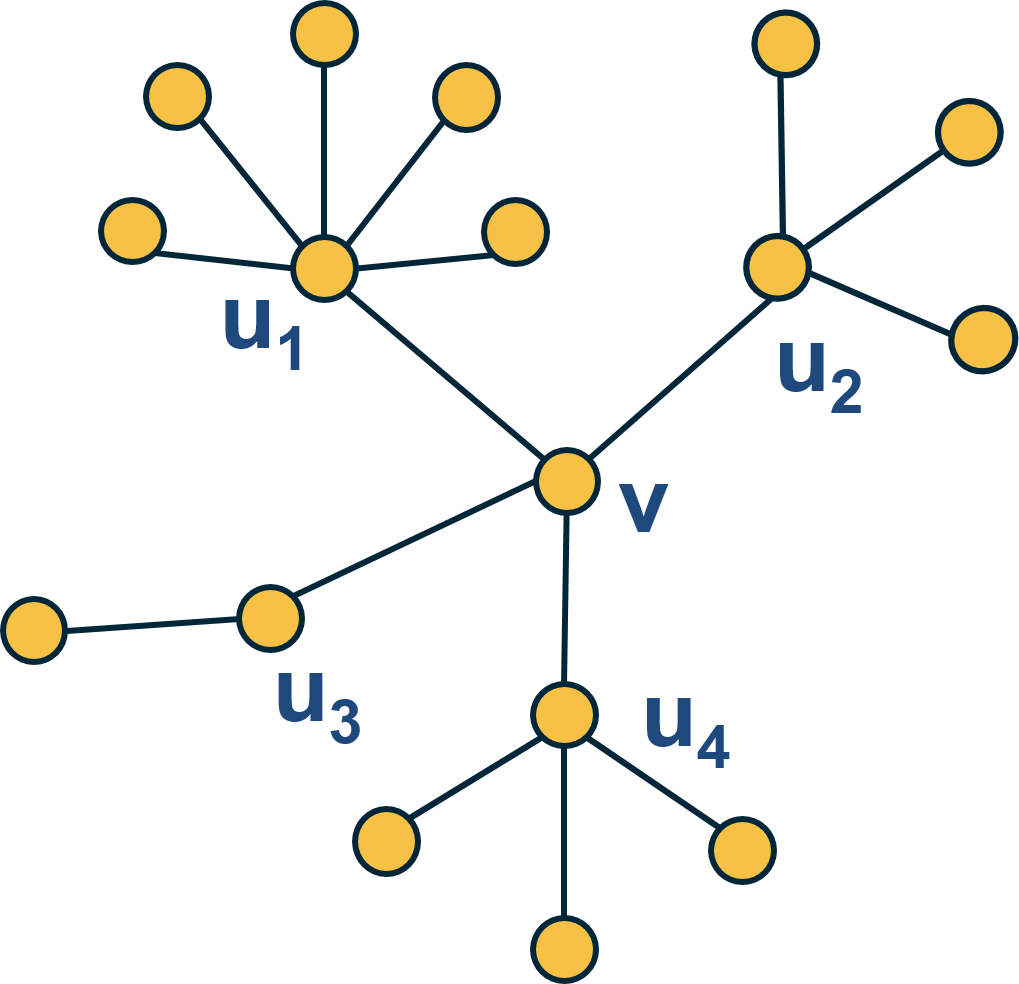
\includegraphics[width=0.5\linewidth]{k-neighbor-example.png}
    \caption{    $\overline{k_{nn}}\left(v\right)\:=\frac{\:1}{k\left(v\right)}\sum_{i=1}^{k\left(v\right)}k\left(u_i\right)=\frac{6+4+2+4}{4}\:=\:4$}
\end{figure}
Terms Network Science vs. Graph Theory
\begin{table}
\centering

\begin{tabular}{|l|l|}
\hline
\textbf{Network Science} & \textbf{Graph Theory}\\
\hline

\hline
Network & Graph  \\
\hline
Node & Vertex  \\
\hline
Link & Edge  \\
\hline

\end{tabular}

\end{table}


\newpage
\section{Neutral Network}
Definition: the Degree of any two notes is not correlated.
\textbf{Most networks are not Neutral}
$k_{nn}(k)\:=\:\overline{k}+\frac{\sigma_k^2}{\overline{k}}=\bar{k}_{nn}$
\newpage
\section{The \textit{G(n,p)} model (ER Graphs) Erdős–Rényi}
This is the simplest random graph. It is not the same as the $G(N,L)$ graph, which has a fixed number of random links.
\subsection{Construction}
\begin{description}
    \item [n] Nodes
    \item [p] the probability any two nodes are connected 
\end{description}

\subsection{Properties}
Note how the LCC suddenly 'explodes' when the average node degree is greater than 1. This is called a phase transition. 
\begin{figure}
    \centering
    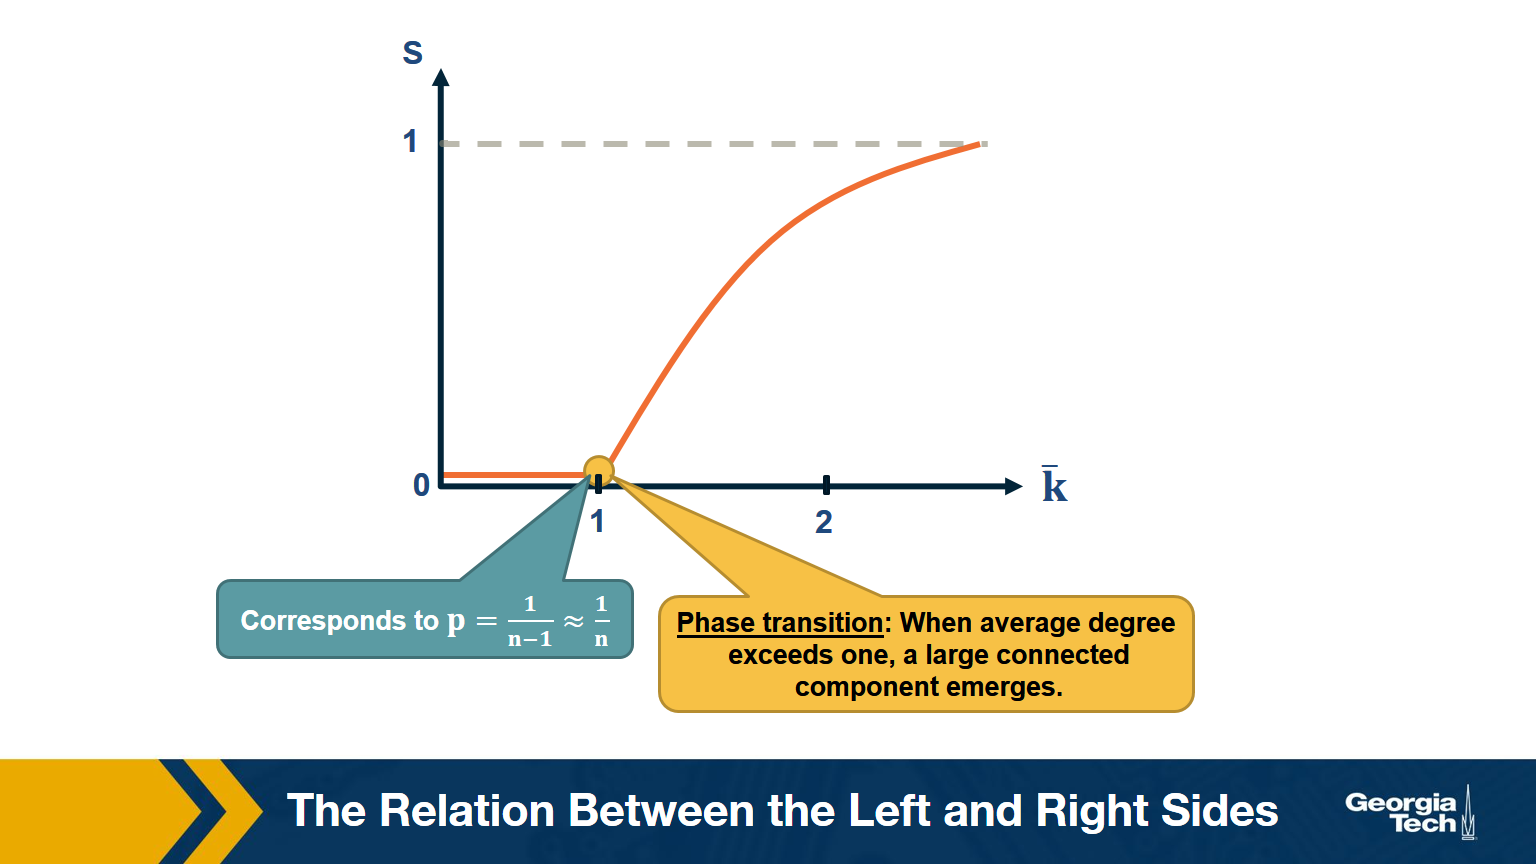
\includegraphics[width=1\linewidth]{lcc-explosion.png}
\end{figure}
\begin{description}
    \item [Degree Distribution]  $p_k\:=\:e^{-\overline{k}}\cdot{\frac{\overline{k}^{k}}{k!}},\:k=0,1,2,\dots$
    \item [average edges] $p\cdot{\binom{n}{2}}$
    \item [edges] expected number of edges is  $|E|=p\cdot\frac{n(n-1)}{2}$
    \item[LCC] Largest Connected Component
    \item[Link Count $P_L$] = $ P(Link Count = L) =( {\begin{array}{*{20}c} {\frac{{N(N - 1)}}{2}}  \\ L  \\ \end{array}} )p^L (1 - p)^{\frac{{N(N - 1)}}{2} - L}$
    \item [S] the probability that a node belongs to LCC\\
    $\overline{S} = S-1$ represents the probability that a node is \textbf{not} connected to a LCC
    $\overline{S}\:=\:((1-p)\:+\:p\cdot\overline{S})^{n-1}$\\
    $1-p$   Probability that a node is not connected to a randomly chosen other node.\\
    $p\cdot\overline{S}$ Probability that the node connects to a node \textbf{not in} the giant component. 
    \item [average node degree] $p\cdot(n-1)$
    \item [average neighbor degree] at a $G(n,p)$ network is\\
    $\overline{k_{nn}}=\overline{k}\:+\:(1-p)$ using the Binomial distribution) or\\
    $\overline{k_{nn}}=\overline{k}\:+\:(1-p)$ using the Poisson approximation when $p\ll1$
\end{description}
\textbf{Question: how large should $p$ (or $k$) be so that the LCC covers all network nodes?  }

Answer: The probability that a node does \textbf{not} connect to any node in the LCC $\left(1-p\right)^{S \, n}\approx\left(1-p\right)^n\:$if$\:S\approx1$

The expected number of nodes not connecting to LCC:
$\:n\cdot\left(1-p\right)^n\:=\:n\left(1-\frac{np}{n}\right)^n\approx n\cdot e^{-np}$

Limit Definition of Exponential Function $\left(1-\frac{x}{n}\right)^n\approx e^{-x}$
\subsection{links}
\href{https://en.wikipedia.org/wiki/Erd%C5%91s%E2%80%93R%C3%A9nyi_model}{wikipedia}\\
\href{https://en.wikipedia.org/wiki/Binomial_distribution}{Binomial distribution}\\
The Puissant distribution is a good approximation when $n>1,000$

\section{Resources}
\href{https://gatech.instructure.com/courses/433540/modules}{Course Modules}
\href{https://cazabetremy.fr/Teaching/CN2021/CheatSheet/CN_CS_introduction.pdf}{Cheatsheet}


\end{document}
